\section{what is fog computing}
With the rise in smart applications and demand to decrease the latency between the info generation
and processing stage, Cisco coined a brand new term referred to as the fog computing. Fog computing
is the extension of cloud computing towards the network edge to alter cloud-things service time.
It is supported the principle that processing and communication  to be served nearer to the
data sources. Fog computing allows smart applications to perform their processes on network devices which can be routers, gateways or switches instead of causing information to cloud information centers.The principle assures the matter of resource scarcity in IoT as expensive storage, computation and management, and networking may be well offloaded to close fog nodes. This continuously will increase the effectiveness and latency of smart applications. like all services, security mechanisms in IoT can be enforced and deployed at fog layer level, having fog nodes as a proxy, to dump costly storage and computations from IoT devices. Thus, fog nodes give a novel chance for IoT in deploying distributed and collaborative security mechanisms. As compared with cloud computing, fog computing devices can provide less latency for the smart application .
\section{Architecture of fog computing environment}

Fig 1.1 provides a layered architecture of fog computing environment with different devices involved in it. The lowest layer of this architecture contains the data generation devices which can be sensors, RFID tags, cameras, Internet of Things (IoT) devices and actuators. These devices will generate real-time data which should be processed by a smart application to make real-time decisions. Middle layer of the architecture consists of the network devices used to send the data from lower layer devices to the cloud computing infrastructure. This layer can act as a fog layer part or whole computation can be processed so that the application performance is not affected by the latency of the network. Devices in the fog layer are called edge device.
The upper layer is the cloud layer which consists of virtual machines which can be provisioned from any of the cloud service provider. If fog layer does not have free computational resources then it can send the re-quests directly to the cloud infrastructure.
\begin{figure}[h]
	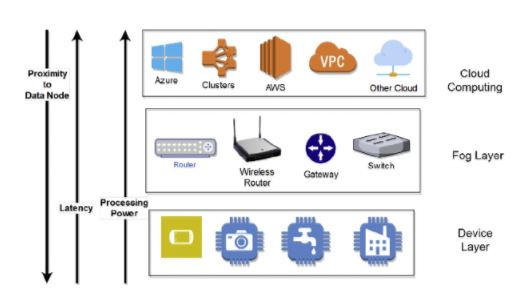
\includegraphics[width=\linewidth]{Capture9.JPG}
	\caption{}
	\label{fig:boat1}
\end{figure}
\section{security in fog computing}
Device security is one in every of the most important challenges for efficient implementation of internet of Things and fog computing atmosphere in current IT house. In fog computing, for any instance of your time same edge device will be utilized by multiple smart applications with totally different set of users that increases the difficulty level of security of edge device. If edge device is hacked, it will get false input and supply false output data, and formulate unnecessary results which  have an effect on the performance of entire application. Hacked device also  want to share information and results with competitive firms or radical teams concerned in unwanted activities. Security protocols that is used currently a days certify every edge device with the application before providing information or computation to perform.

\subsection*{Types of attacks in fog computing}
 If edge device is hacked then scenario becomes even worse as a result of that edge device has certain privileges within the network. So the attack by edge devices on the fog computing setting can be generally characterised into 2 main classes that area unit \textbf{(a) unauthenticated attacks} and\textbf{(b) unauthorized attacks.} If the edge device is unauthenticated and tries to attack the device layer or cloud layer then this attack is named unauthenticated attack or outside attack.But, if the edge device that attacks the fog layer or cloud layer is edge and it's within the given network of application then it's referred to as unauthorized or inside attack.
\subsection*{Attack detection in fog computing}
Though fog computing design can give the required service necessities and distributed resources, robust security mechanisms are required resources to shield IoT devices. As preventive security schemes  with the shortcoming design and implementation flaws, detective mechanisms such as attack detections are inevitable. Attack detections will be either signature primarily based or anomaly
based schemes. The signature primarily based answer matches the incoming traffic against the already identified attack varieties within the info whereas anomaly primarily based theme caters for attack detection as a activity deviation
from traditional traffic. the previous approach has been used widely to its high accuracy of detection and low warning rate, however criticized for its incapability to capture novel attacks. Anomaly detection, on the other hand  detects new attacks although it lacks high accuracy. In these approaches, classical machine learning has been used extensively. With the ever increasing  attackers power and
resources, ancient machine learning algorithms are incapable of police work complicated cyber breaches. The fog nodes are answerable for training models and hosting attack detection systems at the edge of the distributed fog network.




 









